\documentclass[12pt,a4paper]{article}
\usepackage[utf8]{inputenc}
\usepackage[german]{babel}
\usepackage[T1]{fontenc}
\usepackage{amsmath}
\usepackage{amsfonts}
\usepackage{amssymb}
\usepackage{graphicx}
\usepackage[left=2.5cm,right=2.5cm,top=2cm,bottom=2cm]{geometry}
\usepackage{float}
\author{Gruppe C14 \\ Julián Häck, Martin Koytek, Lars Wenning, Erik Zimmermann}
\begin{document}
\section{Dichtigkeitsmessung - Vorversuch}
\subsection{Versuchsbeschreibung}
Wir vermessen die Dichtigkeit unserer im Hauptversuch verwendeten Apparatur mit Hilfe des Drucksensors und einer Handpumpe, in dem wir einen für den Hauptversuch typischen Unterdruck erzeugen ($\approx$300 hPa) und die Leckrate messen. Wir tragen die Werte für den Druck gegen die Zeit auf und ermitteln die Leckrate (in $\frac{hPa}{min}$) mittels einer Linearen Regression.

\subsection{Versuchsaufbau und Durchführung}
Wir verwenden den selben Versuchsaufbau wie im Hauptversuch, jedoch fügen wir eine Handpumpe dem T-Ventil hinzu. Die Messwerterfassungseinstellung ändern sich nicht gegenüber den anderen Vorversuchen.
Wir erzeugen mit Hilfe der Handpumpe einen Unterdruck und messen den Druck über 10 Minuten. Dieser nimmt linear über die Zeit hinweg zu. Wir messen den Druck und tragen diesen gegen die Zeit auf.
\subsection{Versuchsauswertung}

\subsubsection{Rohdaten}

\begin{figure}[H]
\centering
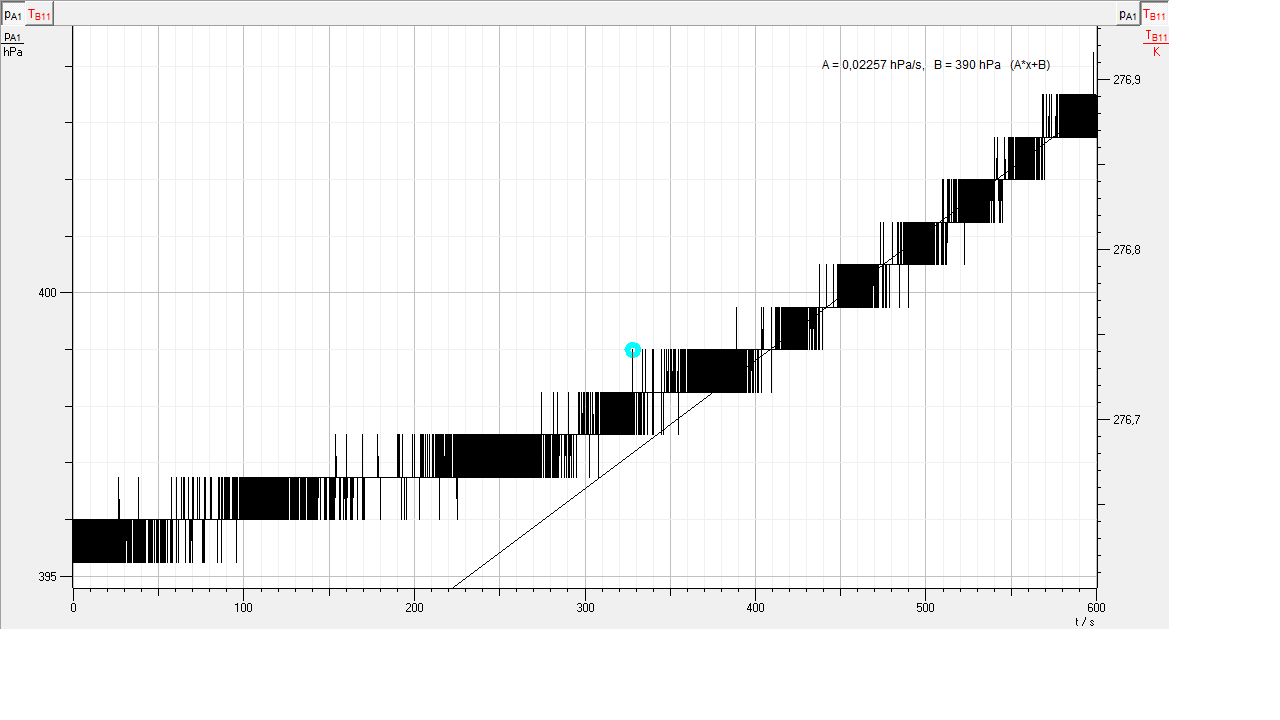
\includegraphics[scale=0.3]{Bilder/dichtigkeit_raw_JM.png}
\caption{Leckmessung Gruppe 1}
\end{figure}

\begin{figure}[H]
\centering
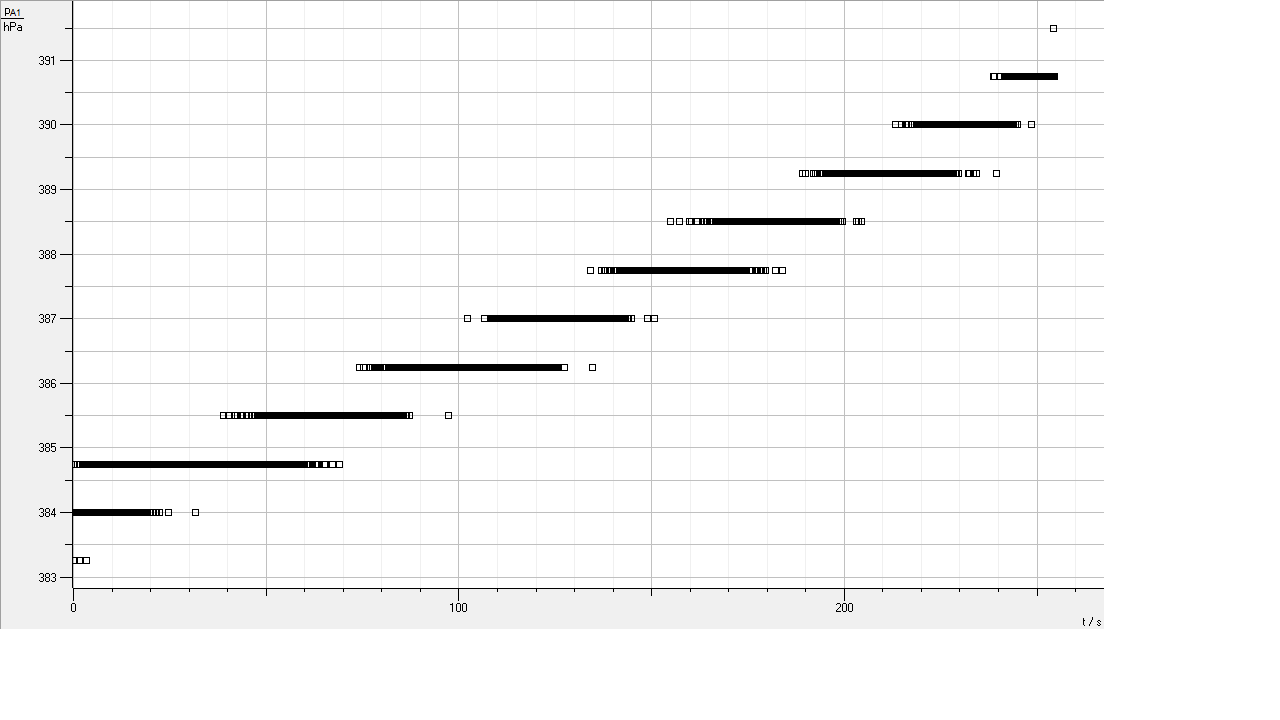
\includegraphics[scale=0.3]{Bilder/dichtigkeit_raw_EL.png}
\caption{Leckmessung Gruppe 2}
\end{figure}

\subsubsection{Transformation und Analyse der Rohdaten}

Bei Gruppe 1 haben wir am Anfang eine sich ändernde Leckrate festgestellt, die zunächst bei $\approx$0.7$\,\frac{hPa}{min}$ lag. Diese pendelte sich gegen Ende der Messung bei 1.264$\,\frac{hPa}{min}$ ein. Daher haben wir vor der Linearen Regression die Werte vom Anfang abgeschnitten. Wir führen eine Lineare Regression durch und erhalten aus der Steigung die Leckrate.

\begin{figure}[H]
\centering
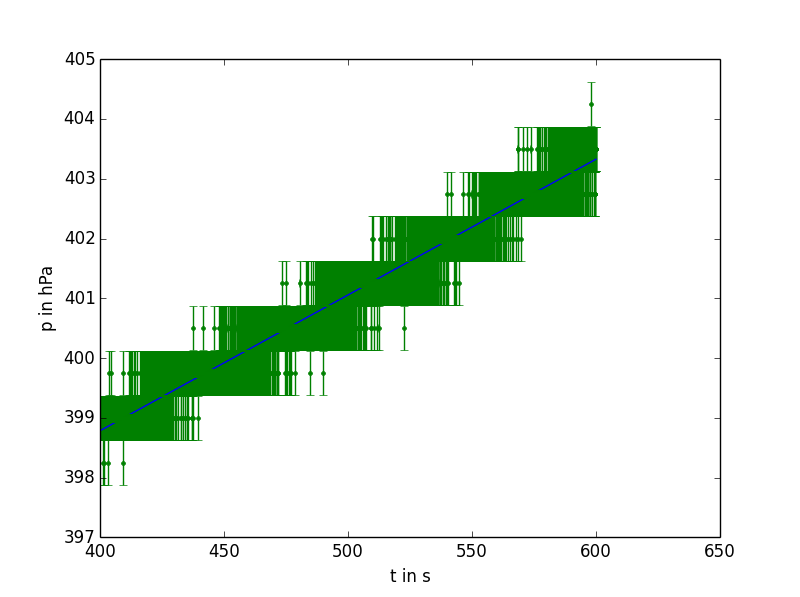
\includegraphics[scale=0.5]{Bilder/dichtigkeit__JM.png}
\caption{Lineare Regression Gruppe 1 $\frac{\chi^2}{f}=0.638$}
\end{figure}

\begin{figure}[H]
\centering
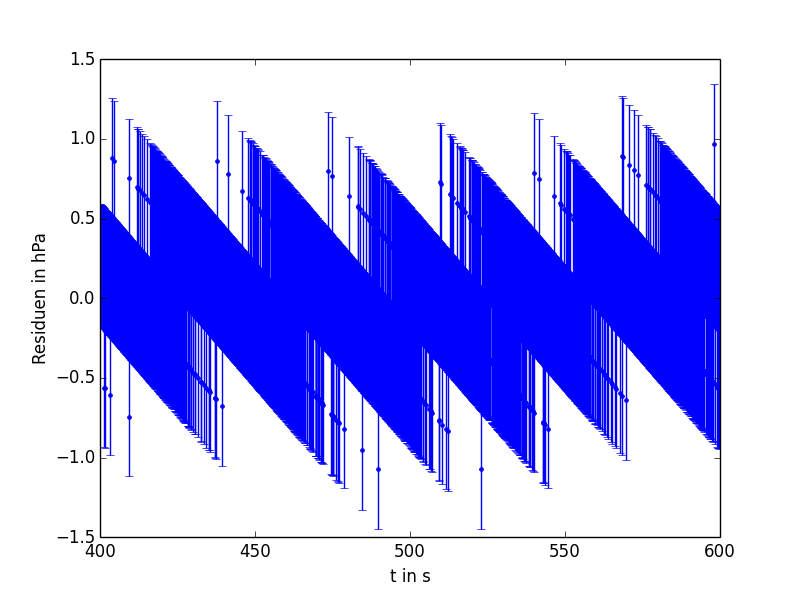
\includegraphics[scale=0.5]{Bilder/residuen_dichtigkeit_JM.png}
\caption{Residuen für die Anpassung von Gruppe 1}
\end{figure}

Die Leckrate für Gruppe 1 beträgt 1.364$\,\frac{hPa}{min}$.
\newpage

\begin{figure}[H]
\centering
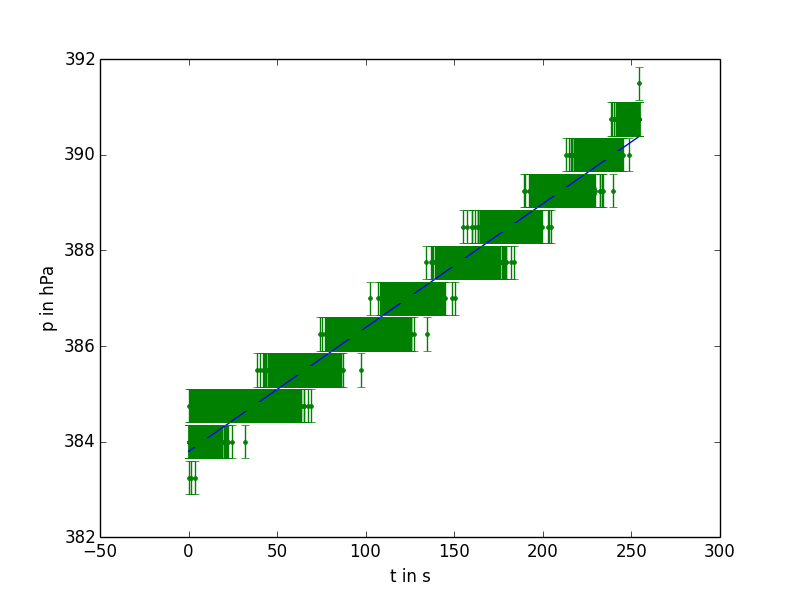
\includegraphics[scale=0.5]{Bilder/dichtigkeit__EL.png}
\caption{Lineare Regression Gruppe 2, $\frac{\chi^2}{f}=0.804$}
\end{figure}

\begin{figure}[H]
\centering
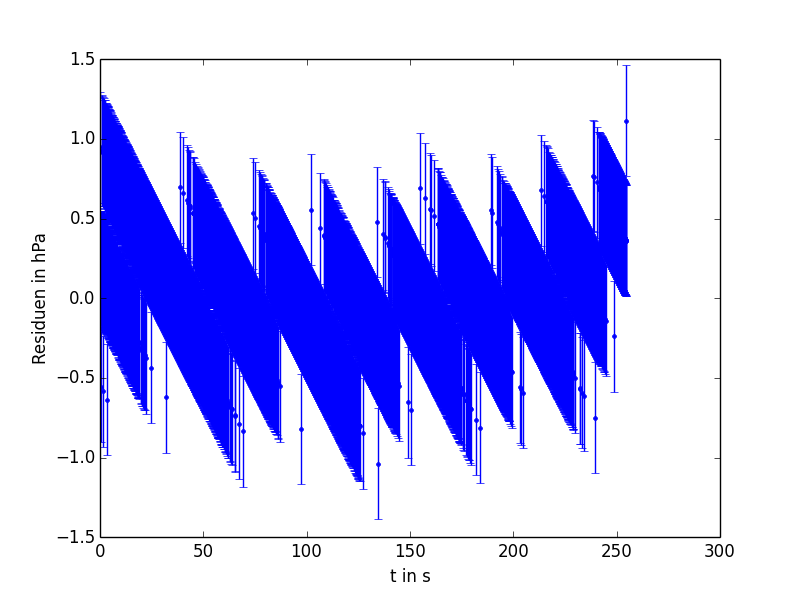
\includegraphics[scale=0.5]{Bilder/residuen_dichtigkeit_EL.png}
\caption{Residuen der Anpassung Gruppe 2}
\end{figure}

Die Leckrate für Gruppe 2 beträgt 1.554$\,\frac{hPa}{min}$.

\subsubsection{Fazit}
Die Leckraten von 1.364$\,\frac{hPa}{min}$, bzw 1.554$\,\frac{hPa}{min}$ betragen nur ca $\frac{1}{300}$ unseres eigentlichen Wertes. Da die Lineare Regression in einem Bereich stattgefunden hat, in dem wir mir der Aulösung des Sensors arbeiten mussten, sieht man diese Bereich sehr gut in den Residuenplots. Ansonsten lassen sich keine Systematiken feststellen. Wir sind mit den Ergebnissen des Vorversuchs zufrieden, die Güte der Anpassung liegt ebenfalls in einem zufriedenstellenden Rahmen ($\frac{\chi^2}{f}=0.638$ für Gruppe 1 und $\frac{\chi^2}{f}=0.804$ für Gruppe 2).
\end{document}